\section{Basic concepts}

%%================================================================================
%%
\subsection{Terminology}
%%
%%================================================================================
\begin{frame}
    \frametitle{\secname: \small\subsecname\normalsize}

    \begin{itemize}
        \item The \textbf{Workspace} is where you can work with a set of files
        \begin{itemize}
            \item Regardless of whether those files are being tracked or not
            \item Modify files
            \item Build something with the file
            \item Etc
        \end{itemize}
        \item A \textbf{Version} is a recorded state of the tracked set of files
        \begin{itemize}
            \item A Version doesn't need to be named
            \item A single commit may be considered a version
        \end{itemize}
        \item A \textbf{Repository} is the entire set of files and every recorded version (also possibly accompanying meta-data)
        \item \textbf{To check out} is the act of retrieve a file (or a set of files) from the repository to the workspace
    \end{itemize}
\end{frame}

%%================================================================================
%%
\subsection{Version Control System (VCS)}
%%
%%================================================================================
\begin{frame}
    \frametitle{\secname: \small\subsecname\normalsize}

    Version control is a system that records changes to a file or set of files over time so that you can recall specific versions later.

    \begin{itemize}
        \item Local VCS
        \item Centralized VCS
        \item Distributed VCS
    \end{itemize}
\end{frame}

%%================================================================================
%%
\subsection{VCS - Local VCS}
%%
%%================================================================================
\begin{frame}
    \frametitle{\secname: \small\subsecname\normalsize}

    Simplest VCS of them all: copy files from one directory to another directory.

    \begin{figure}[h]
        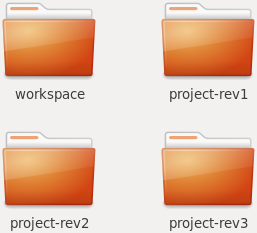
\includegraphics[height=0.5\textheight]{000-vcs-local-repo}
        \centering
    \end{figure}
\end{frame}

%%================================================================================
%%
\subsection{VCS - Centralized VCS}
%%
%%================================================================================
\begin{frame}
    \frametitle{\secname: \small\subsecname\normalsize}

    A single (usually?) remote entity stores and manages the repository.

    \begin{figure}[h]
        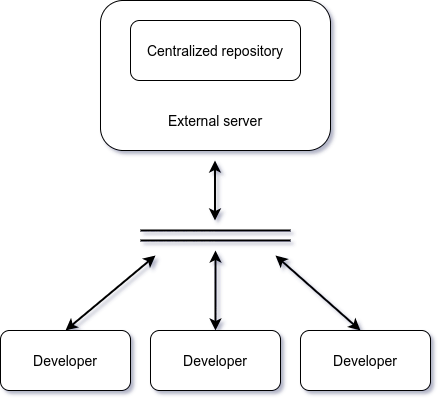
\includegraphics[height=0.6\textheight]{000-vcs-centralized.png}
        \centering
    \end{figure}
\end{frame}

\begin{frame}
    \frametitle{\secname: \small\subsecname\normalsize}

    \begin{columns}
        % Left side
        \column{0.35\textwidth}
            \begin{figure}[h]
                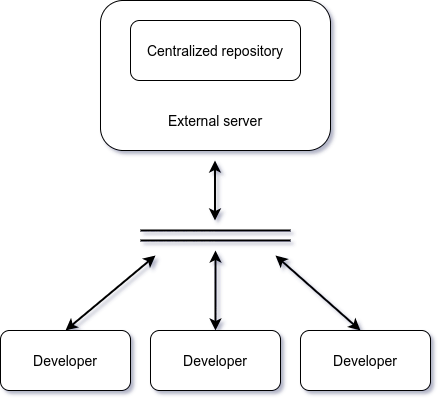
\includegraphics[width=\textwidth]{000-vcs-centralized.png}
                \centering
            \end{figure}

        % Right side
        \column{0.65\textwidth}
            \begin{itemize}
                \item Only the centralizing entity has a copy of the entire repository
                \item Every operation requires communicating with the centralizing entity
                \begin{itemize}
                    \item Checking out a specific version
                    \item Committing new versions
                    \item Checking the history of the repository
                    \item Etc.
                \end{itemize}
            \end{itemize}
    \end{columns}
\end{frame}

%%================================================================================
%%
\subsection{VCS - Distributed VCS}
%%
%%================================================================================
\begin{frame}
    \frametitle{\secname: \small\subsecname\normalsize}

    Everyone has a copy of the entire repository.

    \begin{figure}[h]
        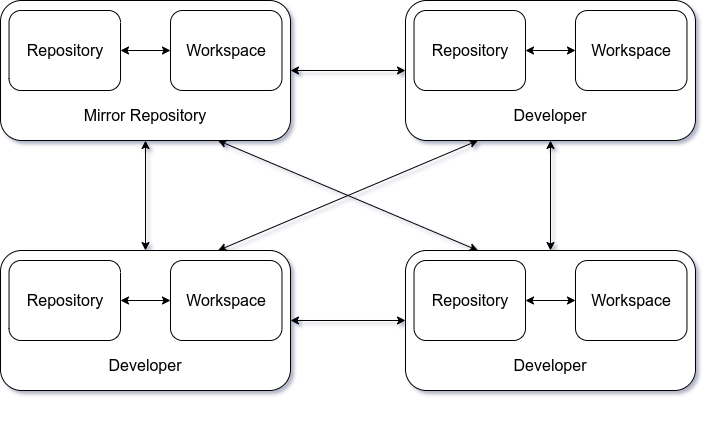
\includegraphics[width=\textwidth]{000-vcs-distributed-plain}
        \centering
    \end{figure}
\end{frame}

\begin{frame}
    \frametitle{\secname: \small\subsecname\normalsize}

    \begin{columns}
        % Left side
        \column{0.35\textwidth}

        \begin{figure}[h]
            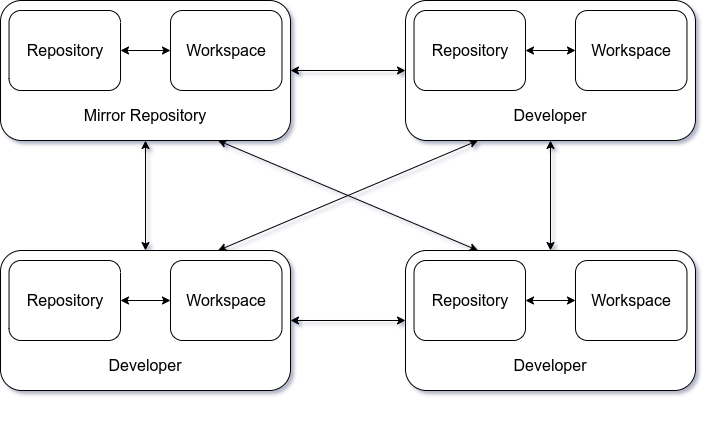
\includegraphics[width=\textwidth]{000-vcs-distributed-plain}
            \centering
        \end{figure}

        % Right side
        \column{0.65\textwidth}
            \begin{itemize}
                \item Most operations may be done in the local repository
                \begin{itemize}
                    \item Checking out a specific (and previously downloaded) version
                    \item Committing new versions
                    \item Checking the (downloaded) history of the repository
                    \item Etc.
                \end{itemize}
                \item New versions may be pushed or retrieve to remote repositories
            \end{itemize}
    \end{columns}
\end{frame}

\begin{frame}
    \frametitle{\secname: \small\subsecname\normalsize}

    One entity (or more) may be selected as the "official" repository

    \begin{figure}[h]
        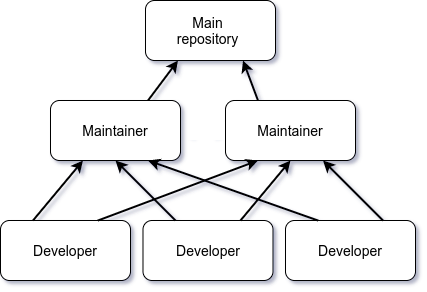
\includegraphics[width=0.75\textwidth]{000-vcs-distributed-hierarchy}
        \centering
    \end{figure}
\end{frame}
